\section{Early detection of potential dropout students}

\label{sec:strategy}

This way, the problem we address in this paper consists of a strategy to \textit{early} identify potential failing students. Notice that identifying early is very important in the sense that professors still have enough time to act and avoid students to fail the course. This way, we focus exclusively on early identifying these students. Providing or reporting a technique useful to reduce the failure rate is outside the scope of this paper. Nevertheless, notice that when identifying them we may study the data and afterwards provide a technique to do so. Actually, based on the results of this paper, we intend to propose a technique to reduce the failure rate as future work.

Next, we detail our strategy to identify these students.

\subsection{Online exercises system}
% This section should answer: Why is this kind of system important to identify potential falling students?
% Answer: We need metrics. In order to discover how students are performing, it is necessary a close monitoring of students behaviour
% Talk about Huxley, only enough to explain the metrics: submissions and submission_status (Correct ...)

As a side effect, we believe that this kind of system will be useful to improve the overall performance of students:
% #1 Students only learn how to program programming, a lot ... 
% #2 Students need rapid feedback
% #3 Students learn at different speed
% #4 There always be great students and bad students, then the great should be presented to challenges that make them even greater and the bad ones should be presented to a different set of problems that allow them to become better


% The Huxley is an online exercise system that has features that provides all these needs (then, it will justify our choice )


To evaluate the students performance during the course, we use an online exercises system named Huxley~\cite{}. \todo{algum texto ja pronto?}

Problem-solving approach

The more practice the more learning

Programming is learned by programming, not from books~\cite{}.
The Huxley allows student to avoid the ``learned helplessness'' problems. This problem happens when a student who has missed a basic concept and who then cannot follow the next lecture. She believes that there is no going back; the course is behaving very much as a high-speed train with no brakes. Such a student will quickly come to the view that ``they just can't do programming'', and will attribute this to the perceived difficulty of the subject.

\subsection{Metrics}

\label{sec:metrics}

We use two metrics in our strategy. We explain them in what follows:

\begin{itemize}

	\item \textbf{Number of submissions:} this metric represents the number of submissions a student do during the course. As explained, Huxley provides more than 300 programming exercises. To solve a particular problem, a student needs to submit at least one solution.

	\item \textbf{Number of correct submissions:} if a student solves one problem, we increase this metric by one.

\end{itemize}

Depending on the level of difficulty of a problem, students may submit several times to solve it. However, notice that this is not necessarily a bad thing regarding the learning process. For example, submitting many times means that students are somehow practicing and studying continuously. Thus, although she is not hitting a right solution, she is trying hard and will eventually hit one. Nevertheless, we need to carefully analyze \todots

\todo{Por que essas metricas sao boas? Por que escolhemos elas? O texto acima ajuda a explicar isso? Essas metricas nao sao obvias?}

\subsection{Clustering algorithm}

To identify potential failing students, we use the well-known clustering algorithm k-means~\cite{}. As input, we set the algorithm to compute three groups. To compute the groups, the algorithm takes into account the metrics we present in Section~\ref{sec:metrics}.

We choose three groups because ???

\todo{Por que escolhemos clustering? Por que o k-means?}

\todo{Por que 3 grupos? O do meio seria impossível prever algo. Mas isso nao e obvio?}

\subsection{Summary}

Figure~\ref{fig:strategy} combines all steps of our strategy. As the classes are happening, students are encouraged to solve exercises using the problems of Huxley. Although solving exercises is not mandatory, there some particular activities where the professor forces students to use Huxley. Next, we collect the metrics we detail in Section~\ref{sec:metrics}. To identify potential failing students \textit{early}, we collect the metrics for the first 30 days of the introductory programming courses. Then, we execute the k-means clustering algorithm.

%Then, we execute a R script we implemented to execute the clustering algorithm. As can be seen, there are three groups, represented by circles, squares, and stars. \todo{falar dos 30 dias}

\begin{figure}[htb]
\centering
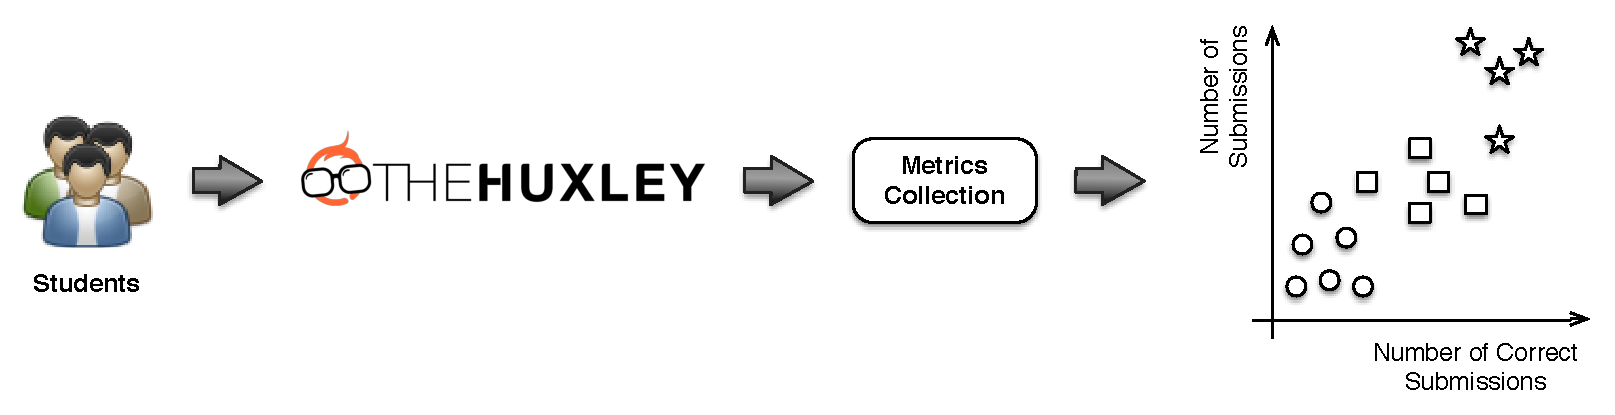
\includegraphics[width=1.0\textwidth,natwidth=610,natheight=642]{images/Strategy.pdf}
\caption{Summary of our strategy to identify potential failing students.}
\label{fig:strategy}
\end{figure}